%  \begin{figure}[htb]	
%  \center%6.3
%  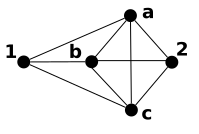
\includegraphics[width=5cm]{./img/lemaClaw2Maximais.png}
%  \caption{Example of Construction 1 }
% \label{fig:lemaClaw2Maximais}
% \end{figure}  
 
 
 
\begin{figure}[ht]
  \centering
  \begin{tabular}{  p{5cm} p{0.7cm} p{5cm} }
    %\centering
    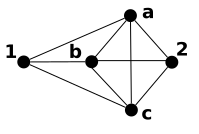
\includegraphics[width=3.5cm]{img/lemaClaw2Maximais} & &
    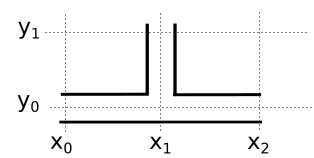
\includegraphics[width=5.5cm]{img/claw2}
    \\
    \footnotesize %\centering 
    (a)  \footnotesize Example of two maximal cliques sharing vertices. && \footnotesize (b) Representation  of a claw-clique in grid.\\
  \end{tabular}

 \caption{Vertices represented by a claw are present in a unique maximal clique.} \label{fig:lemaClaw2Maximais}
\end{figure}